\documentclass[1p]{elsarticle_modified}
%\bibliographystyle{elsarticle-num}

%\usepackage[colorlinks]{hyperref}
%\usepackage{abbrmath_seonhwa} %\Abb, \Ascr, \Acal ,\Abf, \Afrak
\usepackage{amsfonts}
\usepackage{amssymb}
\usepackage{amsmath}
\usepackage{amsthm}
\usepackage{scalefnt}
\usepackage{amsbsy}
\usepackage{kotex}
\usepackage{caption}
\usepackage{subfig}
\usepackage{color}
\usepackage{graphicx}
\usepackage{xcolor} %% white, black, red, green, blue, cyan, magenta, yellow
\usepackage{float}
\usepackage{setspace}
\usepackage{hyperref}

\usepackage{tikz}
\usetikzlibrary{arrows}

\usepackage{multirow}
\usepackage{array} % fixed length table
\usepackage{hhline}

%%%%%%%%%%%%%%%%%%%%%
\makeatletter
\renewcommand*\env@matrix[1][\arraystretch]{%
	\edef\arraystretch{#1}%
	\hskip -\arraycolsep
	\let\@ifnextchar\new@ifnextchar
	\array{*\c@MaxMatrixCols c}}
\makeatother %https://tex.stackexchange.com/questions/14071/how-can-i-increase-the-line-spacing-in-a-matrix
%%%%%%%%%%%%%%%

\usepackage[normalem]{ulem}

\newcommand{\msout}[1]{\ifmmode\text{\sout{\ensuremath{#1}}}\else\sout{#1}\fi}
%SOURCE: \msout is \stkout macro in https://tex.stackexchange.com/questions/20609/strikeout-in-math-mode

\newcommand{\cancel}[1]{
	\ifmmode
	{\color{red}\msout{#1}}
	\else
	{\color{red}\sout{#1}}
	\fi
}

\newcommand{\add}[1]{
	{\color{blue}\uwave{#1}}
}

\newcommand{\replace}[2]{
	\ifmmode
	{\color{red}\msout{#1}}{\color{blue}\uwave{#2}}
	\else
	{\color{red}\sout{#1}}{\color{blue}\uwave{#2}}
	\fi
}

\newcommand{\Sol}{\mathcal{S}} %segment
\newcommand{\D}{D} %diagram
\newcommand{\A}{\mathcal{A}} %arc


%%%%%%%%%%%%%%%%%%%%%%%%%%%%%5 test

\def\sl{\operatorname{\textup{SL}}(2,\Cbb)}
\def\psl{\operatorname{\textup{PSL}}(2,\Cbb)}
\def\quan{\mkern 1mu \triangleright \mkern 1mu}

\theoremstyle{definition}
\newtheorem{thm}{Theorem}[section]
\newtheorem{prop}[thm]{Proposition}
\newtheorem{lem}[thm]{Lemma}
\newtheorem{ques}[thm]{Question}
\newtheorem{cor}[thm]{Corollary}
\newtheorem{defn}[thm]{Definition}
\newtheorem{exam}[thm]{Example}
\newtheorem{rmk}[thm]{Remark}
\newtheorem{alg}[thm]{Algorithm}

\newcommand{\I}{\sqrt{-1}}
\begin{document}

%\begin{frontmatter}
%
%\title{Boundary parabolic representations of knots up to 8 crossings}
%
%%% Group authors per affiliation:
%\author{Yunhi Cho} 
%\address{Department of Mathematics, University of Seoul, Seoul, Korea}
%\ead{yhcho@uos.ac.kr}
%
%
%\author{Seonhwa Kim} %\fnref{s_kim}}
%\address{Center for Geometry and Physics, Institute for Basic Science, Pohang, 37673, Korea}
%\ead{ryeona17@ibs.re.kr}
%
%\author{Hyuk Kim}
%\address{Department of Mathematical Sciences, Seoul National University, Seoul 08826, Korea}
%\ead{hyukkim@snu.ac.kr}
%
%\author{Seokbeom Yoon}
%\address{Department of Mathematical Sciences, Seoul National University, Seoul, 08826,  Korea}
%\ead{sbyoon15@snu.ac.kr}
%
%\begin{abstract}
%We find all boundary parabolic representation of knots up to 8 crossings.
%
%\end{abstract}
%\begin{keyword}
%    \MSC[2010] 57M25 
%\end{keyword}
%
%\end{frontmatter}

%\linenumbers
%\tableofcontents
%
\newcommand\colored[1]{\textcolor{white}{\rule[-0.35ex]{0.8em}{1.4ex}}\kern-0.8em\color{red} #1}%
%\newcommand\colored[1]{\textcolor{white}{ #1}\kern-2.17ex	\textcolor{white}{ #1}\kern-1.81ex	\textcolor{white}{ #1}\kern-2.15ex\color{red}#1	}

{\Large $\underline{12a_{0904}~(K12a_{0904})}$}

\setlength{\tabcolsep}{10pt}
\renewcommand{\arraystretch}{1.6}
\vspace{1cm}\begin{tabular}{m{100pt}>{\centering\arraybackslash}m{274pt}}
\multirow{5}{120pt}{
	\centering
	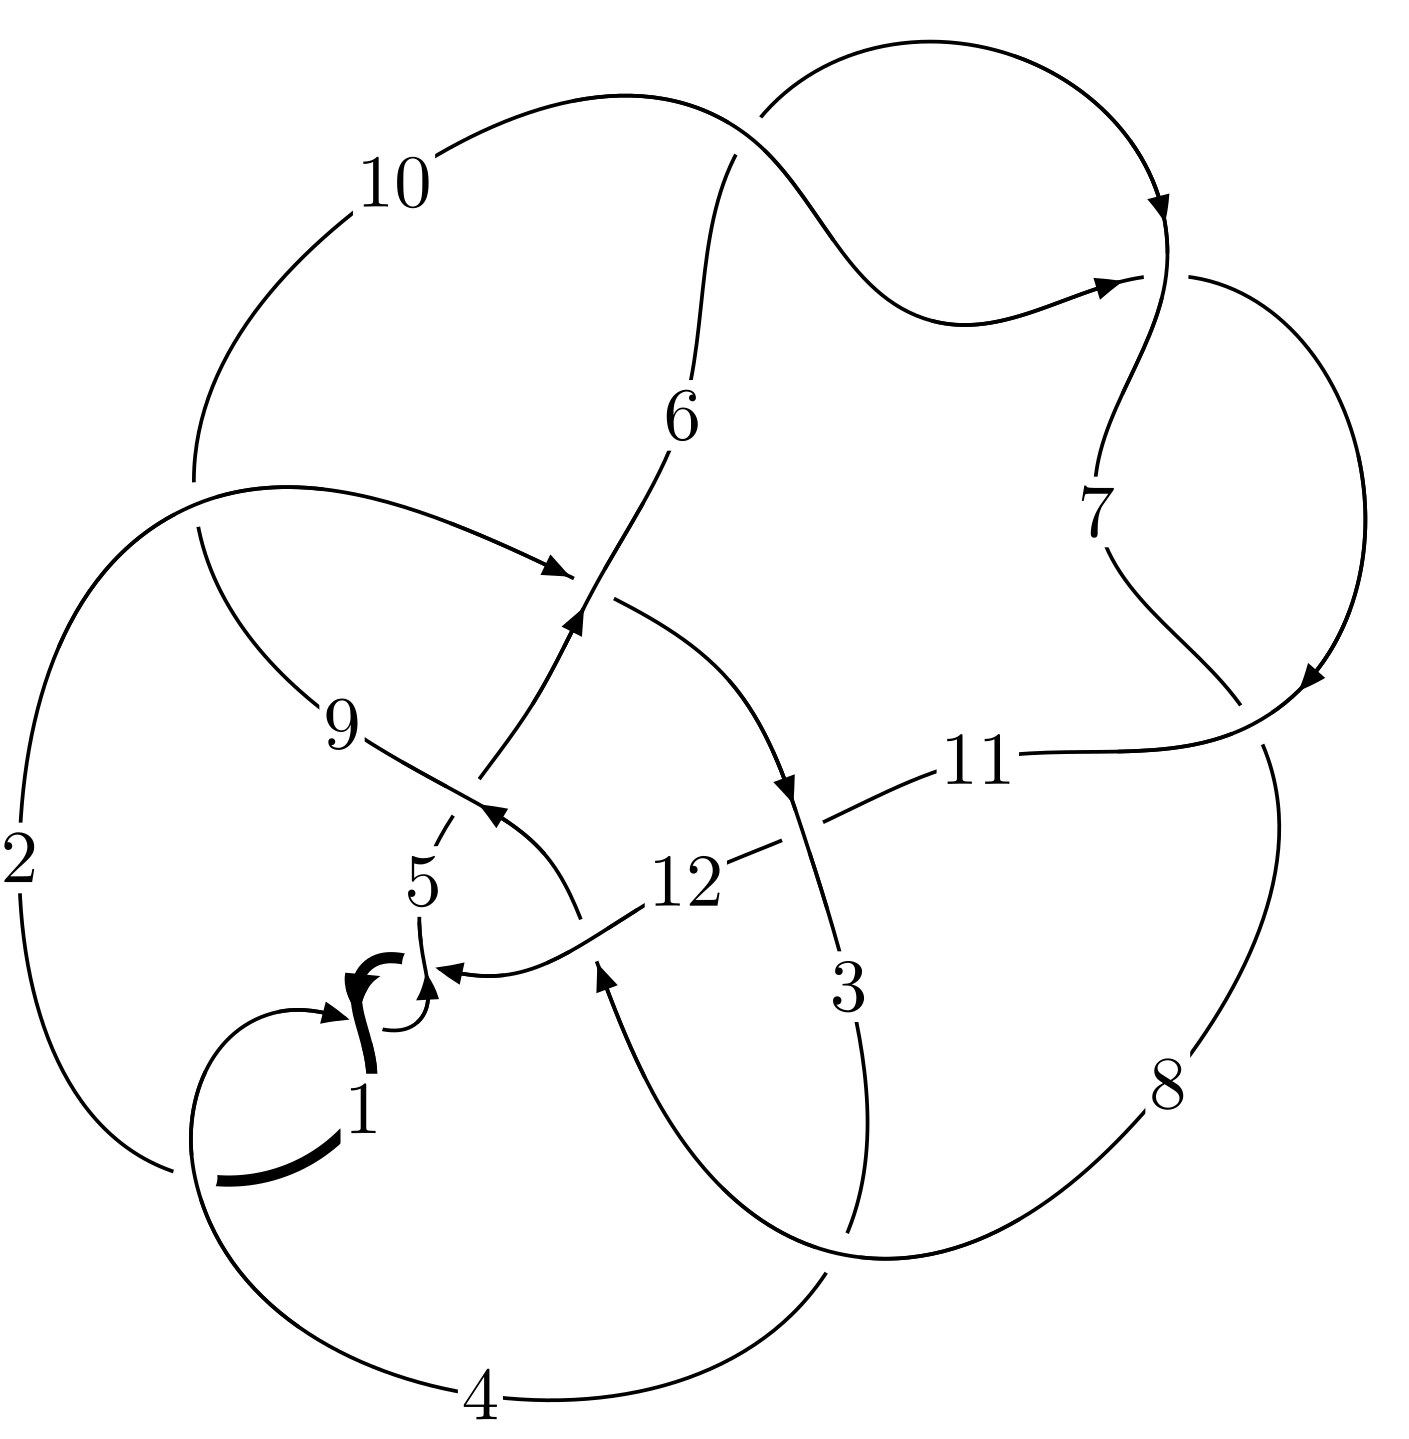
\includegraphics[width=112pt]{../../../GIT/diagram.site/Diagrams/png/1705_12a_0904.png}\\
\ \ \ A knot diagram\footnotemark}&
\allowdisplaybreaks
\textbf{Linearized knot diagam} \\
\cline{2-2}
 &
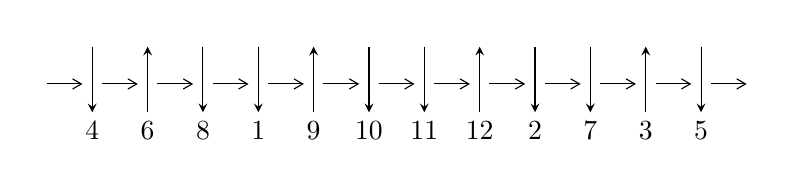
\begin{tikzpicture}[x=20pt, y=17pt]
	% nodes
	\node (C0) at (0, 0) {};
	\node (C1) at (1, 0) {};
	\node (C1U) at (1, +1) {};
	\node (C1D) at (1, -1) {4};

	\node (C2) at (2, 0) {};
	\node (C2U) at (2, +1) {};
	\node (C2D) at (2, -1) {6};

	\node (C3) at (3, 0) {};
	\node (C3U) at (3, +1) {};
	\node (C3D) at (3, -1) {8};

	\node (C4) at (4, 0) {};
	\node (C4U) at (4, +1) {};
	\node (C4D) at (4, -1) {1};

	\node (C5) at (5, 0) {};
	\node (C5U) at (5, +1) {};
	\node (C5D) at (5, -1) {9};

	\node (C6) at (6, 0) {};
	\node (C6U) at (6, +1) {};
	\node (C6D) at (6, -1) {10};

	\node (C7) at (7, 0) {};
	\node (C7U) at (7, +1) {};
	\node (C7D) at (7, -1) {11};

	\node (C8) at (8, 0) {};
	\node (C8U) at (8, +1) {};
	\node (C8D) at (8, -1) {12};

	\node (C9) at (9, 0) {};
	\node (C9U) at (9, +1) {};
	\node (C9D) at (9, -1) {2};

	\node (C10) at (10, 0) {};
	\node (C10U) at (10, +1) {};
	\node (C10D) at (10, -1) {7};

	\node (C11) at (11, 0) {};
	\node (C11U) at (11, +1) {};
	\node (C11D) at (11, -1) {3};

	\node (C12) at (12, 0) {};
	\node (C12U) at (12, +1) {};
	\node (C12D) at (12, -1) {5};
	\node (C13) at (13, 0) {};

	% arrows
	\draw[->,>={angle 60}]
	(C0) edge (C1) (C1) edge (C2) (C2) edge (C3) (C3) edge (C4) (C4) edge (C5) (C5) edge (C6) (C6) edge (C7) (C7) edge (C8) (C8) edge (C9) (C9) edge (C10) (C10) edge (C11) (C11) edge (C12) (C12) edge (C13) ;	\draw[->,>=stealth]
	(C1U) edge (C1D) (C2D) edge (C2U) (C3U) edge (C3D) (C4U) edge (C4D) (C5D) edge (C5U) (C6U) edge (C6D) (C7U) edge (C7D) (C8D) edge (C8U) (C9U) edge (C9D) (C10U) edge (C10D) (C11D) edge (C11U) (C12U) edge (C12D) ;
	\end{tikzpicture} \\
\hhline{~~} \\& 
\textbf{Solving Sequence} \\ \cline{2-2} 
 &
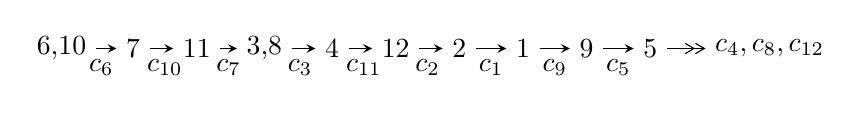
\begin{tikzpicture}[x=23pt, y=7pt]
	% node
	\node (A0) at (-1/8, 0) {6,10};
	\node (A1) at (1, 0) {7};
	\node (A2) at (2, 0) {11};
	\node (A3) at (49/16, 0) {3,8};
	\node (A4) at (33/8, 0) {4};
	\node (A5) at (41/8, 0) {12};
	\node (A6) at (49/8, 0) {2};
	\node (A7) at (57/8, 0) {1};
	\node (A8) at (65/8, 0) {9};
	\node (A9) at (73/8, 0) {5};
	\node (C1) at (1/2, -1) {$c_{6}$};
	\node (C2) at (3/2, -1) {$c_{10}$};
	\node (C3) at (5/2, -1) {$c_{7}$};
	\node (C4) at (29/8, -1) {$c_{3}$};
	\node (C5) at (37/8, -1) {$c_{11}$};
	\node (C6) at (45/8, -1) {$c_{2}$};
	\node (C7) at (53/8, -1) {$c_{1}$};
	\node (C8) at (61/8, -1) {$c_{9}$};
	\node (C9) at (69/8, -1) {$c_{5}$};
	\node (A10) at (11, 0) {$c_{4},c_{8},c_{12}$};

	% edge
	\draw[->,>=stealth]	
	(A0) edge (A1) (A1) edge (A2) (A2) edge (A3) (A3) edge (A4) (A4) edge (A5) (A5) edge (A6) (A6) edge (A7) (A7) edge (A8) (A8) edge (A9) ;
	\draw[->>,>={angle 60}]	
	(A9) edge (A10);
\end{tikzpicture} \\ 

\end{tabular} \\

\footnotetext{
The image of knot diagram is generated by the software ``\textbf{Draw programme}" developed by Andrew Bartholomew(\url{http://www.layer8.co.uk/maths/draw/index.htm\#Running-draw}), where we modified some parts for our purpose(\url{https://github.com/CATsTAILs/LinksPainter}).
}\phantom \\ \newline 
\centering \textbf{Ideals for irreducible components\footnotemark of $X_{\text{par}}$} 
 
\begin{align*}
I^u_{1}&=\langle 
-6.80736\times10^{21} u^{48}+8.45127\times10^{22} u^{47}+\cdots+9.47444\times10^{18} b-6.36777\times10^{22},\\
\phantom{I^u_{1}}&\phantom{= \langle  }-9.78381\times10^{22} u^{48}+1.20822\times10^{24} u^{47}+\cdots+1.42117\times10^{20} a-8.78994\times10^{23},\\
\phantom{I^u_{1}}&\phantom{= \langle  }u^{49}-14 u^{48}+\cdots+15 u-15\rangle \\
I^u_{2}&=\langle 
15 u^{32}+51 u^{31}+\cdots+4 b+29,\;29 u^{32} a-51 u^{32}+\cdots+59 a-55,\;u^{33}+4 u^{32}+\cdots+4 u+1\rangle \\
I^u_{3}&=\langle 
212 u^{18}+746 u^{17}+\cdots+b-143,\;284 u^{18}+993 u^{17}+\cdots+a-188,\;u^{19}+5 u^{18}+\cdots+2 u-1\rangle \\
I^u_{4}&=\langle 
b+1,\;a^4+2 a^3- a^2-2 a+3,\;u-1\rangle \\
I^u_{5}&=\langle 
b-1,\;a^2- a-1,\;u-1\rangle \\
\\
I^v_{1}&=\langle 
a,\;b+1,\;v-1\rangle \\
\end{align*}
\raggedright * 6 irreducible components of $\dim_{\mathbb{C}}=0$, with total 141 representations.\\
\footnotetext{All coefficients of polynomials are rational numbers. But the coefficients are sometimes approximated in decimal forms when there is not enough margin.}
\newpage
\renewcommand{\arraystretch}{1}
\centering \section*{I. $I^u_{1}= \langle -6.81\times10^{21} u^{48}+8.45\times10^{22} u^{47}+\cdots+9.47\times10^{18} b-6.37\times10^{22},\;-9.78\times10^{22} u^{48}+1.21\times10^{24} u^{47}+\cdots+1.42\times10^{20} a-8.79\times10^{23},\;u^{49}-14 u^{48}+\cdots+15 u-15 \rangle$}
\flushleft \textbf{(i) Arc colorings}\\
\begin{tabular}{m{7pt} m{180pt} m{7pt} m{180pt} }
\flushright $a_{6}=$&$\begin{pmatrix}1\\0\end{pmatrix}$ \\
\flushright $a_{10}=$&$\begin{pmatrix}0\\u\end{pmatrix}$ \\
\flushright $a_{7}=$&$\begin{pmatrix}1\\u^2\end{pmatrix}$ \\
\flushright $a_{11}=$&$\begin{pmatrix}- u\\- u^3+u\end{pmatrix}$ \\
\flushright $a_{3}=$&$\begin{pmatrix}688.436 u^{48}-8501.60 u^{47}+\cdots-2513.66 u+6185.02\\718.497 u^{48}-8920.08 u^{47}+\cdots-2579.49 u+6721.00\end{pmatrix}$ \\
\flushright $a_{8}=$&$\begin{pmatrix}- u^2+1\\- u^4+2 u^2\end{pmatrix}$ \\
\flushright $a_{4}=$&$\begin{pmatrix}464.635 u^{48}-5815.98 u^{47}+\cdots-1526.92 u+4698.07\\105.044 u^{48}-1301.83 u^{47}+\cdots-294.460 u+1043.20\end{pmatrix}$ \\
\flushright $a_{12}=$&$\begin{pmatrix}-1047.35 u^{48}+13271.5 u^{47}+\cdots+2929.33 u-11815.0\\-455.203 u^{48}+5771.76 u^{47}+\cdots+1265.32 u-5159.50\end{pmatrix}$ \\
\flushright $a_{2}=$&$\begin{pmatrix}-30.0619 u^{48}+418.482 u^{47}+\cdots+65.8259 u-535.978\\718.497 u^{48}-8920.08 u^{47}+\cdots-2579.49 u+6721.00\end{pmatrix}$ \\
\flushright $a_{1}=$&$\begin{pmatrix}-868.372 u^{48}+10931.9 u^{47}+\cdots+2757.74 u-9184.05\\-367.877 u^{48}+4676.46 u^{47}+\cdots+980.968 u-4262.61\end{pmatrix}$ \\
\flushright $a_{9}=$&$\begin{pmatrix}1011.69 u^{48}-12824.6 u^{47}+\cdots-2762.90 u+11491.1\\790.230 u^{48}-10008.2 u^{47}+\cdots-2225.63 u+8882.16\end{pmatrix}$ \\
\flushright $a_{5}=$&$\begin{pmatrix}158.515 u^{48}-2047.43 u^{47}+\cdots-269.436 u+2139.17\\1034.37 u^{48}-13113.2 u^{47}+\cdots-2833.39 u+11749.5\end{pmatrix}$\\&\end{tabular}
\flushleft \textbf{(ii) Obstruction class $= -1$}\\~\\
\flushleft \textbf{(iii) Cusp Shapes $= \frac{15967610317655355889704}{9474437016710709037} u^{48}-\frac{200050054562027319399210}{9474437016710709037} u^{47}+\cdots-\frac{55240295833948105225005}{9474437016710709037} u+\frac{160054166406768266614452}{9474437016710709037}$}\\~\\
\newpage\renewcommand{\arraystretch}{1}
\flushleft \textbf{(iv) u-Polynomials at the component}\newline \\
\begin{tabular}{m{50pt}|m{274pt}}
Crossings & \hspace{64pt}u-Polynomials at each crossing \\
\hline $$\begin{aligned}c_{1},c_{4},c_{12}\end{aligned}$$&$\begin{aligned}
&u^{49}-9 u^{48}+\cdots-75 u+15
\end{aligned}$\\
\hline $$\begin{aligned}c_{2},c_{11}\end{aligned}$$&$\begin{aligned}
&u^{49}+2 u^{48}+\cdots-12 u-3
\end{aligned}$\\
\hline $$\begin{aligned}c_{3},c_{9}\end{aligned}$$&$\begin{aligned}
&u^{49}-6 u^{47}+\cdots-35 u-11
\end{aligned}$\\
\hline $$\begin{aligned}c_{5},c_{8}\end{aligned}$$&$\begin{aligned}
&u^{49}+4 u^{48}+\cdots-3 u-1
\end{aligned}$\\
\hline $$\begin{aligned}c_{6},c_{7},c_{10}\end{aligned}$$&$\begin{aligned}
&u^{49}+14 u^{48}+\cdots+15 u+15
\end{aligned}$\\
\hline
\end{tabular}\\~\\
\newpage\renewcommand{\arraystretch}{1}
\flushleft \textbf{(v) Riley Polynomials at the component}\newline \\
\begin{tabular}{m{50pt}|m{274pt}}
Crossings & \hspace{64pt}Riley Polynomials at each crossing \\
\hline $$\begin{aligned}c_{1},c_{4},c_{12}\end{aligned}$$&$\begin{aligned}
&y^{49}+47 y^{48}+\cdots+3495 y-225
\end{aligned}$\\
\hline $$\begin{aligned}c_{2},c_{11}\end{aligned}$$&$\begin{aligned}
&y^{49}-6 y^{48}+\cdots+120 y-9
\end{aligned}$\\
\hline $$\begin{aligned}c_{3},c_{9}\end{aligned}$$&$\begin{aligned}
&y^{49}-12 y^{48}+\cdots+1005 y-121
\end{aligned}$\\
\hline $$\begin{aligned}c_{5},c_{8}\end{aligned}$$&$\begin{aligned}
&y^{49}-42 y^{48}+\cdots+141 y-1
\end{aligned}$\\
\hline $$\begin{aligned}c_{6},c_{7},c_{10}\end{aligned}$$&$\begin{aligned}
&y^{49}-54 y^{48}+\cdots+1245 y-225
\end{aligned}$\\
\hline
\end{tabular}\\~\\
\newpage\flushleft \textbf{(vi) Complex Volumes and Cusp Shapes}
$$\begin{array}{c|c|c}  
\text{Solutions to }I^u_{1}& \I (\text{vol} + \sqrt{-1}CS) & \text{Cusp shape}\\
 \hline 
\begin{aligned}
u &= -0.433047 + 0.879529 I \\
a &= \phantom{-}0.291430 + 0.391337 I \\
b &= \phantom{-}0.597708 - 0.538193 I\end{aligned}
 & \phantom{-}1.03664 - 4.43730 I & \phantom{-0.000000 } 0 \\ \hline\begin{aligned}
u &= -0.433047 - 0.879529 I \\
a &= \phantom{-}0.291430 - 0.391337 I \\
b &= \phantom{-}0.597708 + 0.538193 I\end{aligned}
 & \phantom{-}1.03664 + 4.43730 I & \phantom{-0.000000 } 0 \\ \hline\begin{aligned}
u &= -0.615786 + 0.757323 I \\
a &= -0.367363 + 0.678499 I \\
b &= \phantom{-}0.991856 + 0.906798 I\end{aligned}
 & \phantom{-}0.46282 + 9.75261 I & \phantom{-0.000000 } 0 \\ \hline\begin{aligned}
u &= -0.615786 - 0.757323 I \\
a &= -0.367363 - 0.678499 I \\
b &= \phantom{-}0.991856 - 0.906798 I\end{aligned}
 & \phantom{-}0.46282 - 9.75261 I & \phantom{-0.000000 } 0 \\ \hline\begin{aligned}
u &= -0.590062 + 0.843539 I \\
a &= \phantom{-}0.443919 - 0.597588 I \\
b &= -0.998349 - 0.951834 I\end{aligned}
 & \phantom{-}6.6188 + 13.7974 I & \phantom{-0.000000 } 0 \\ \hline\begin{aligned}
u &= -0.590062 - 0.843539 I \\
a &= \phantom{-}0.443919 + 0.597588 I \\
b &= -0.998349 + 0.951834 I\end{aligned}
 & \phantom{-}6.6188 - 13.7974 I & \phantom{-0.000000 } 0 \\ \hline\begin{aligned}
u &= -0.584945 + 0.950148 I \\
a &= -0.331095 - 0.287711 I \\
b &= -0.601232 + 0.675624 I\end{aligned}
 & \phantom{-}6.74131 - 7.96419 I & \phantom{-0.000000 } 0 \\ \hline\begin{aligned}
u &= -0.584945 - 0.950148 I \\
a &= -0.331095 + 0.287711 I \\
b &= -0.601232 - 0.675624 I\end{aligned}
 & \phantom{-}6.74131 + 7.96419 I & \phantom{-0.000000 } 0 \\ \hline\begin{aligned}
u &= -0.725664 + 0.466170 I \\
a &= \phantom{-}0.696467 + 0.277718 I \\
b &= \phantom{-}1.038160 - 0.508456 I\end{aligned}
 & \phantom{-}7.88801 + 1.77959 I & \phantom{-0.000000 } 0 \\ \hline\begin{aligned}
u &= -0.725664 - 0.466170 I \\
a &= \phantom{-}0.696467 - 0.277718 I \\
b &= \phantom{-}1.038160 + 0.508456 I\end{aligned}
 & \phantom{-}7.88801 - 1.77959 I & \phantom{-0.000000 } 0\\
 \hline 
 \end{array}$$\newpage$$\begin{array}{c|c|c}  
\text{Solutions to }I^u_{1}& \I (\text{vol} + \sqrt{-1}CS) & \text{Cusp shape}\\
 \hline 
\begin{aligned}
u &= -0.570337 + 0.621546 I \\
a &= \phantom{-}0.317455 - 0.880503 I \\
b &= -1.009850 - 0.870823 I\end{aligned}
 & \phantom{-}1.36125 + 4.73215 I & \phantom{-0.000000 } 0. - 6.17410 I \\ \hline\begin{aligned}
u &= -0.570337 - 0.621546 I \\
a &= \phantom{-}0.317455 + 0.880503 I \\
b &= -1.009850 + 0.870823 I\end{aligned}
 & \phantom{-}1.36125 - 4.73215 I & \phantom{-0.000000 -}0. + 6.17410 I \\ \hline\begin{aligned}
u &= \phantom{-}0.289625 + 0.769569 I \\
a &= \phantom{-}0.291612 - 0.422229 I \\
b &= -0.369416 + 0.242506 I\end{aligned}
 & \phantom{-}2.10039 - 1.64969 I & \phantom{-0.000000 -}0. + 3.17462 I \\ \hline\begin{aligned}
u &= \phantom{-}0.289625 - 0.769569 I \\
a &= \phantom{-}0.291612 + 0.422229 I \\
b &= -0.369416 - 0.242506 I\end{aligned}
 & \phantom{-}2.10039 + 1.64969 I & \phantom{-0.000000 } 0. - 3.17462 I \\ \hline\begin{aligned}
u &= \phantom{-}1.242710 + 0.016595 I \\
a &= \phantom{-}1.16528 + 1.29445 I \\
b &= \phantom{-}0.319236 + 0.418793 I\end{aligned}
 & \phantom{-}3.15210 + 0.59306 I & \phantom{-0.000000 } 0 \\ \hline\begin{aligned}
u &= \phantom{-}1.242710 - 0.016595 I \\
a &= \phantom{-}1.16528 - 1.29445 I \\
b &= \phantom{-}0.319236 - 0.418793 I\end{aligned}
 & \phantom{-}3.15210 - 0.59306 I & \phantom{-0.000000 } 0 \\ \hline\begin{aligned}
u &= -0.345736 + 0.608967 I \\
a &= -0.681550 + 1.075440 I \\
b &= \phantom{-}1.043400 + 0.803583 I\end{aligned}
 & \phantom{-}8.99740 + 2.00742 I & \phantom{-}3.69703 - 4.15633 I \\ \hline\begin{aligned}
u &= -0.345736 - 0.608967 I \\
a &= -0.681550 - 1.075440 I \\
b &= \phantom{-}1.043400 - 0.803583 I\end{aligned}
 & \phantom{-}8.99740 - 2.00742 I & \phantom{-}3.69703 + 4.15633 I \\ \hline\begin{aligned}
u &= \phantom{-}1.346140 + 0.047168 I \\
a &= -0.443611 - 1.201140 I \\
b &= -0.109835 - 0.592401 I\end{aligned}
 & -2.79905 + 0.29382 I & \phantom{-0.000000 } 0 \\ \hline\begin{aligned}
u &= \phantom{-}1.346140 - 0.047168 I \\
a &= -0.443611 + 1.201140 I \\
b &= -0.109835 + 0.592401 I\end{aligned}
 & -2.79905 - 0.29382 I & \phantom{-0.000000 } 0\\
 \hline 
 \end{array}$$\newpage$$\begin{array}{c|c|c}  
\text{Solutions to }I^u_{1}& \I (\text{vol} + \sqrt{-1}CS) & \text{Cusp shape}\\
 \hline 
\begin{aligned}
u &= -0.350884 + 0.523383 I \\
a &= -0.515791 - 0.746507 I \\
b &= -0.768093 + 0.310045 I\end{aligned}
 & \phantom{-}1.91939 - 0.70956 I & \phantom{-}1.318828 + 0.280442 I \\ \hline\begin{aligned}
u &= -0.350884 - 0.523383 I \\
a &= -0.515791 + 0.746507 I \\
b &= -0.768093 - 0.310045 I\end{aligned}
 & \phantom{-}1.91939 + 0.70956 I & \phantom{-}1.318828 - 0.280442 I \\ \hline\begin{aligned}
u &= -1.42373\phantom{ +0.000000I} \\
a &= -0.459235\phantom{ +0.000000I} \\
b &= -1.58471\phantom{ +0.000000I}\end{aligned}
 & -3.37509\phantom{ +0.000000I} & \phantom{-0.000000 } 0 \\ \hline\begin{aligned}
u &= -1.43526 + 0.05673 I \\
a &= \phantom{-}0.470759 - 0.012708 I \\
b &= \phantom{-}1.64110 - 0.14774 I\end{aligned}
 & \phantom{-}1.28248 + 0.95897 I & \phantom{-0.000000 } 0 \\ \hline\begin{aligned}
u &= -1.43526 - 0.05673 I \\
a &= \phantom{-}0.470759 + 0.012708 I \\
b &= \phantom{-}1.64110 + 0.14774 I\end{aligned}
 & \phantom{-}1.28248 - 0.95897 I & \phantom{-0.000000 } 0 \\ \hline\begin{aligned}
u &= -1.44574 + 0.13037 I \\
a &= -0.285354 - 0.092403 I \\
b &= -1.051010 - 0.180394 I\end{aligned}
 & -3.51728 + 4.30782 I & \phantom{-0.000000 } 0 \\ \hline\begin{aligned}
u &= -1.44574 - 0.13037 I \\
a &= -0.285354 + 0.092403 I \\
b &= -1.051010 + 0.180394 I\end{aligned}
 & -3.51728 - 4.30782 I & \phantom{-0.000000 } 0 \\ \hline\begin{aligned}
u &= \phantom{-}1.44985 + 0.18119 I \\
a &= \phantom{-}0.29317 - 2.09746 I \\
b &= \phantom{-}0.90354 - 1.19821 I\end{aligned}
 & \phantom{-}3.18263 - 4.79396 I & \phantom{-0.000000 } 0 \\ \hline\begin{aligned}
u &= \phantom{-}1.44985 - 0.18119 I \\
a &= \phantom{-}0.29317 + 2.09746 I \\
b &= \phantom{-}0.90354 + 1.19821 I\end{aligned}
 & \phantom{-}3.18263 + 4.79396 I & \phantom{-0.000000 } 0 \\ \hline\begin{aligned}
u &= \phantom{-}1.47749 + 0.03978 I \\
a &= -0.19780 + 2.30854 I \\
b &= -0.31875 + 1.60961 I\end{aligned}
 & -6.62186 - 2.92931 I & \phantom{-0.000000 } 0\\
 \hline 
 \end{array}$$\newpage$$\begin{array}{c|c|c}  
\text{Solutions to }I^u_{1}& \I (\text{vol} + \sqrt{-1}CS) & \text{Cusp shape}\\
 \hline 
\begin{aligned}
u &= \phantom{-}1.47749 - 0.03978 I \\
a &= -0.19780 - 2.30854 I \\
b &= -0.31875 - 1.60961 I\end{aligned}
 & -6.62186 + 2.92931 I & \phantom{-0.000000 } 0 \\ \hline\begin{aligned}
u &= -1.49311\phantom{ +0.000000I} \\
a &= \phantom{-}0.281474\phantom{ +0.000000I} \\
b &= \phantom{-}1.04778\phantom{ +0.000000I}\end{aligned}
 & -7.43487\phantom{ +0.000000I} & \phantom{-0.000000 } 0 \\ \hline\begin{aligned}
u &= \phantom{-}0.479702\phantom{ +0.000000I} \\
a &= -1.05468\phantom{ +0.000000I} \\
b &= \phantom{-}0.263235\phantom{ +0.000000I}\end{aligned}
 & -0.947319\phantom{ +0.000000I} & -10.8700\phantom{ +0.000000I} \\ \hline\begin{aligned}
u &= \phantom{-}1.54367 + 0.20987 I \\
a &= -0.37262 + 1.86764 I \\
b &= -1.11448 + 1.32193 I\end{aligned}
 & -5.62131 - 7.81657 I & \phantom{-0.000000 } 0 \\ \hline\begin{aligned}
u &= \phantom{-}1.54367 - 0.20987 I \\
a &= -0.37262 - 1.86764 I \\
b &= -1.11448 - 1.32193 I\end{aligned}
 & -5.62131 + 7.81657 I & \phantom{-0.000000 } 0 \\ \hline\begin{aligned}
u &= \phantom{-}1.56434 + 0.25553 I \\
a &= \phantom{-}0.27338 - 1.74910 I \\
b &= \phantom{-}1.17492 - 1.28124 I\end{aligned}
 & -6.6890 - 13.4975 I & \phantom{-0.000000 } 0 \\ \hline\begin{aligned}
u &= \phantom{-}1.56434 - 0.25553 I \\
a &= \phantom{-}0.27338 + 1.74910 I \\
b &= \phantom{-}1.17492 + 1.28124 I\end{aligned}
 & -6.6890 + 13.4975 I & \phantom{-0.000000 } 0 \\ \hline\begin{aligned}
u &= \phantom{-}1.56308 + 0.29110 I \\
a &= -0.17723 + 1.71857 I \\
b &= -1.20463 + 1.25726 I\end{aligned}
 & -0.3997 - 17.9676 I & \phantom{-0.000000 } 0 \\ \hline\begin{aligned}
u &= \phantom{-}1.56308 - 0.29110 I \\
a &= -0.17723 - 1.71857 I \\
b &= -1.20463 - 1.25726 I\end{aligned}
 & -0.3997 + 17.9676 I & \phantom{-0.000000 } 0 \\ \hline\begin{aligned}
u &= -0.359518 + 0.130940 I \\
a &= \phantom{-}0.10471 - 2.15999 I \\
b &= -0.436809 - 1.042280 I\end{aligned}
 & -0.50334 + 2.29820 I & -0.41049 + 7.94845 I\\
 \hline 
 \end{array}$$\newpage$$\begin{array}{c|c|c}  
\text{Solutions to }I^u_{1}& \I (\text{vol} + \sqrt{-1}CS) & \text{Cusp shape}\\
 \hline 
\begin{aligned}
u &= -0.359518 - 0.130940 I \\
a &= \phantom{-}0.10471 + 2.15999 I \\
b &= -0.436809 + 1.042280 I\end{aligned}
 & -0.50334 - 2.29820 I & -0.41049 - 7.94845 I \\ \hline\begin{aligned}
u &= \phantom{-}1.67836 + 0.27620 I \\
a &= -0.010084 + 0.531761 I \\
b &= -0.356849 + 0.558291 I\end{aligned}
 & -5.86325 - 0.66633 I & \phantom{-0.000000 } 0 \\ \hline\begin{aligned}
u &= \phantom{-}1.67836 - 0.27620 I \\
a &= -0.010084 - 0.531761 I \\
b &= -0.356849 - 0.558291 I\end{aligned}
 & -5.86325 + 0.66633 I & \phantom{-0.000000 } 0 \\ \hline\begin{aligned}
u &= \phantom{-}1.70957 + 0.15400 I \\
a &= \phantom{-}0.077778 - 0.702600 I \\
b &= \phantom{-}0.354253 - 0.806660 I\end{aligned}
 & -1.46119 + 3.06033 I & \phantom{-0.000000 } 0 \\ \hline\begin{aligned}
u &= \phantom{-}1.70957 - 0.15400 I \\
a &= \phantom{-}0.077778 + 0.702600 I \\
b &= \phantom{-}0.354253 + 0.806660 I\end{aligned}
 & -1.46119 - 3.06033 I & \phantom{-0.000000 } 0 \\ \hline\begin{aligned}
u &= \phantom{-}1.67687 + 0.48704 I \\
a &= -0.069085 - 0.340576 I \\
b &= \phantom{-}0.328404 - 0.384973 I\end{aligned}
 & -2.14546 - 4.63461 I & \phantom{-0.000000 } 0 \\ \hline\begin{aligned}
u &= \phantom{-}1.67687 - 0.48704 I \\
a &= -0.069085 + 0.340576 I \\
b &= \phantom{-}0.328404 + 0.384973 I\end{aligned}
 & -2.14546 + 4.63461 I & \phantom{-0.000000 } 0 \\ \hline\begin{aligned}
u &= \phantom{-}0.133847 + 0.185778 I \\
a &= -4.35816 + 3.14536 I \\
b &= \phantom{-}1.083580 + 0.119708 I\end{aligned}
 & \phantom{-}6.62641 - 0.11786 I & \phantom{-}5.86559 - 0.14016 I \\ \hline\begin{aligned}
u &= \phantom{-}0.133847 - 0.185778 I \\
a &= -4.35816 - 3.14536 I \\
b &= \phantom{-}1.083580 - 0.119708 I\end{aligned}
 & \phantom{-}6.62641 + 0.11786 I & \phantom{-}5.86559 + 0.14016 I\\
 \hline 
 \end{array}$$\newpage\newpage\renewcommand{\arraystretch}{1}
\centering \section*{II. $I^u_{2}= \langle 15 u^{32}+51 u^{31}+\cdots+4 b+29,\;29 u^{32} a-51 u^{32}+\cdots+59 a-55,\;u^{33}+4 u^{32}+\cdots+4 u+1 \rangle$}
\flushleft \textbf{(i) Arc colorings}\\
\begin{tabular}{m{7pt} m{180pt} m{7pt} m{180pt} }
\flushright $a_{6}=$&$\begin{pmatrix}1\\0\end{pmatrix}$ \\
\flushright $a_{10}=$&$\begin{pmatrix}0\\u\end{pmatrix}$ \\
\flushright $a_{7}=$&$\begin{pmatrix}1\\u^2\end{pmatrix}$ \\
\flushright $a_{11}=$&$\begin{pmatrix}- u\\- u^3+u\end{pmatrix}$ \\
\flushright $a_{3}=$&$\begin{pmatrix}a\\-3.75000 u^{32}-12.7500 u^{31}+\cdots-14.2500 u-7.25000\end{pmatrix}$ \\
\flushright $a_{8}=$&$\begin{pmatrix}- u^2+1\\- u^4+2 u^2\end{pmatrix}$ \\
\flushright $a_{4}=$&$\begin{pmatrix}u^{32}+5 u^{31}+\cdots+a+4\\-5.75000 u^{32}-16.7500 u^{31}+\cdots-17.2500 u-7.25000\end{pmatrix}$ \\
\flushright $a_{12}=$&$\begin{pmatrix}\frac{15}{4} u^{32} a+7 u^{32}+\cdots+\frac{29}{4} a+4\\1\end{pmatrix}$ \\
\flushright $a_{2}=$&$\begin{pmatrix}\frac{15}{4} u^{32}+\frac{51}{4} u^{31}+\cdots+a+\frac{29}{4}\\-3.75000 u^{32}-12.7500 u^{31}+\cdots-14.2500 u-7.25000\end{pmatrix}$ \\
\flushright $a_{1}=$&$\begin{pmatrix}\frac{1}{4} u^{32} a+\frac{23}{4} u^{32}+\cdots+\frac{5}{4} a+\frac{13}{4}\\\frac{1}{4} u^{32} a+u^{32}+\cdots+\frac{1}{4} a+\frac{3}{2}\end{pmatrix}$ \\
\flushright $a_{9}=$&$\begin{pmatrix}-\frac{3}{4} u^{32} a-\frac{27}{4} u^{32}+\cdots+\frac{7}{4} a-\frac{19}{4}\\\frac{11}{4} u^{32} a+\frac{31}{4} u^{31} a+\cdots+\frac{13}{4} a-1\end{pmatrix}$ \\
\flushright $a_{5}=$&$\begin{pmatrix}\frac{1}{2} u^{31} a+\frac{27}{4} u^{32}+\cdots-\frac{1}{2} a+\frac{15}{4}\\-\frac{5}{4} u^{32} a+\frac{1}{4} u^{32}+\cdots-\frac{3}{4} a+\frac{5}{4}\end{pmatrix}$\\&\end{tabular}
\flushleft \textbf{(ii) Obstruction class $= -1$}\\~\\
\flushleft \textbf{(iii) Cusp Shapes $= -\frac{183}{4} u^{32}-\frac{515}{4} u^{31}+\cdots-\frac{397}{4} u-\frac{289}{4}$}\\~\\
\newpage\renewcommand{\arraystretch}{1}
\flushleft \textbf{(iv) u-Polynomials at the component}\newline \\
\begin{tabular}{m{50pt}|m{274pt}}
Crossings & \hspace{64pt}u-Polynomials at each crossing \\
\hline $$\begin{aligned}c_{1},c_{4},c_{12}\end{aligned}$$&$\begin{aligned}
&(u^{33}+7 u^{32}+\cdots+6 u+2)^{2}
\end{aligned}$\\
\hline $$\begin{aligned}c_{2},c_{11}\end{aligned}$$&$\begin{aligned}
&u^{66}-3 u^{65}+\cdots-422 u+59
\end{aligned}$\\
\hline $$\begin{aligned}c_{3},c_{9}\end{aligned}$$&$\begin{aligned}
&u^{66}-5 u^{64}+\cdots-7821 u+1213
\end{aligned}$\\
\hline $$\begin{aligned}c_{5},c_{8}\end{aligned}$$&$\begin{aligned}
&u^{66}+2 u^{65}+\cdots-195 u-107
\end{aligned}$\\
\hline $$\begin{aligned}c_{6},c_{7},c_{10}\end{aligned}$$&$\begin{aligned}
&(u^{33}-4 u^{32}+\cdots+4 u-1)^{2}
\end{aligned}$\\
\hline
\end{tabular}\\~\\
\newpage\renewcommand{\arraystretch}{1}
\flushleft \textbf{(v) Riley Polynomials at the component}\newline \\
\begin{tabular}{m{50pt}|m{274pt}}
Crossings & \hspace{64pt}Riley Polynomials at each crossing \\
\hline $$\begin{aligned}c_{1},c_{4},c_{12}\end{aligned}$$&$\begin{aligned}
&(y^{33}+33 y^{32}+\cdots+84 y-4)^{2}
\end{aligned}$\\
\hline $$\begin{aligned}c_{2},c_{11}\end{aligned}$$&$\begin{aligned}
&y^{66}+29 y^{65}+\cdots+16970 y+3481
\end{aligned}$\\
\hline $$\begin{aligned}c_{3},c_{9}\end{aligned}$$&$\begin{aligned}
&y^{66}-10 y^{65}+\cdots-30663517 y+1471369
\end{aligned}$\\
\hline $$\begin{aligned}c_{5},c_{8}\end{aligned}$$&$\begin{aligned}
&y^{66}-2 y^{65}+\cdots-846945 y+11449
\end{aligned}$\\
\hline $$\begin{aligned}c_{6},c_{7},c_{10}\end{aligned}$$&$\begin{aligned}
&(y^{33}-34 y^{32}+\cdots+20 y-1)^{2}
\end{aligned}$\\
\hline
\end{tabular}\\~\\
\newpage\flushleft \textbf{(vi) Complex Volumes and Cusp Shapes}
$$\begin{array}{c|c|c}  
\text{Solutions to }I^u_{2}& \I (\text{vol} + \sqrt{-1}CS) & \text{Cusp shape}\\
 \hline 
\begin{aligned}
u &= \phantom{-}0.688220 + 0.730433 I \\
a &= \phantom{-}0.679420 + 0.177115 I \\
b &= -0.390156 + 0.737285 I\end{aligned}
 & \phantom{-}1.96145 - 1.06750 I & -5.04121 - 0.08113 I \\ \hline\begin{aligned}
u &= \phantom{-}0.688220 + 0.730433 I \\
a &= \phantom{-}0.070121 - 0.168584 I \\
b &= -0.172925 - 0.537570 I\end{aligned}
 & \phantom{-}1.96145 - 1.06750 I & -5.04121 - 0.08113 I \\ \hline\begin{aligned}
u &= \phantom{-}0.688220 - 0.730433 I \\
a &= \phantom{-}0.679420 - 0.177115 I \\
b &= -0.390156 - 0.737285 I\end{aligned}
 & \phantom{-}1.96145 + 1.06750 I & -5.04121 + 0.08113 I \\ \hline\begin{aligned}
u &= \phantom{-}0.688220 - 0.730433 I \\
a &= \phantom{-}0.070121 + 0.168584 I \\
b &= -0.172925 + 0.537570 I\end{aligned}
 & \phantom{-}1.96145 + 1.06750 I & -5.04121 + 0.08113 I \\ \hline\begin{aligned}
u &= \phantom{-}0.480050 + 0.852324 I \\
a &= \phantom{-}0.708758 + 0.499855 I \\
b &= -0.697285 + 0.596564 I\end{aligned}
 & \phantom{-}2.63544 - 4.29581 I & -2.69433 + 7.14256 I \\ \hline\begin{aligned}
u &= \phantom{-}0.480050 + 0.852324 I \\
a &= -0.267358 - 0.076310 I \\
b &= \phantom{-}0.280856 - 1.024980 I\end{aligned}
 & \phantom{-}2.63544 - 4.29581 I & -2.69433 + 7.14256 I \\ \hline\begin{aligned}
u &= \phantom{-}0.480050 - 0.852324 I \\
a &= \phantom{-}0.708758 - 0.499855 I \\
b &= -0.697285 - 0.596564 I\end{aligned}
 & \phantom{-}2.63544 + 4.29581 I & -2.69433 - 7.14256 I \\ \hline\begin{aligned}
u &= \phantom{-}0.480050 - 0.852324 I \\
a &= -0.267358 + 0.076310 I \\
b &= \phantom{-}0.280856 + 1.024980 I\end{aligned}
 & \phantom{-}2.63544 + 4.29581 I & -2.69433 - 7.14256 I \\ \hline\begin{aligned}
u &= \phantom{-}0.554324 + 0.780221 I \\
a &= -0.574660 - 0.354350 I \\
b &= \phantom{-}0.531601 - 0.665036 I\end{aligned}
 & -1.79727 - 2.60552 I & -13.6142 + 5.4970 I \\ \hline\begin{aligned}
u &= \phantom{-}0.554324 + 0.780221 I \\
a &= \phantom{-}0.202674 + 0.210448 I \\
b &= -0.201059 + 0.756653 I\end{aligned}
 & -1.79727 - 2.60552 I & -13.6142 + 5.4970 I\\
 \hline 
 \end{array}$$\newpage$$\begin{array}{c|c|c}  
\text{Solutions to }I^u_{2}& \I (\text{vol} + \sqrt{-1}CS) & \text{Cusp shape}\\
 \hline 
\begin{aligned}
u &= \phantom{-}0.554324 - 0.780221 I \\
a &= -0.574660 + 0.354350 I \\
b &= \phantom{-}0.531601 + 0.665036 I\end{aligned}
 & -1.79727 + 2.60552 I & -13.6142 - 5.4970 I \\ \hline\begin{aligned}
u &= \phantom{-}0.554324 - 0.780221 I \\
a &= \phantom{-}0.202674 - 0.210448 I \\
b &= -0.201059 - 0.756653 I\end{aligned}
 & -1.79727 + 2.60552 I & -13.6142 - 5.4970 I \\ \hline\begin{aligned}
u &= \phantom{-}1.104540 + 0.315968 I \\
a &= \phantom{-}1.345920 + 0.217380 I \\
b &= \phantom{-}0.894831 + 0.743190 I\end{aligned}
 & \phantom{-}4.76058 + 1.84769 I & -1.10325 - 3.83345 I \\ \hline\begin{aligned}
u &= \phantom{-}1.104540 + 0.315968 I \\
a &= \phantom{-}0.491156 + 0.257639 I \\
b &= -1.047590 - 0.033948 I\end{aligned}
 & \phantom{-}4.76058 + 1.84769 I & -1.10325 - 3.83345 I \\ \hline\begin{aligned}
u &= \phantom{-}1.104540 - 0.315968 I \\
a &= \phantom{-}1.345920 - 0.217380 I \\
b &= \phantom{-}0.894831 - 0.743190 I\end{aligned}
 & \phantom{-}4.76058 - 1.84769 I & -1.10325 + 3.83345 I \\ \hline\begin{aligned}
u &= \phantom{-}1.104540 - 0.315968 I \\
a &= \phantom{-}0.491156 - 0.257639 I \\
b &= -1.047590 + 0.033948 I\end{aligned}
 & \phantom{-}4.76058 - 1.84769 I & -1.10325 + 3.83345 I \\ \hline\begin{aligned}
u &= \phantom{-}0.790477 + 0.166609 I \\
a &= -0.492307 - 0.049240 I \\
b &= \phantom{-}1.009260 - 0.056854 I\end{aligned}
 & -0.369987 + 0.040866 I & -12.86224 - 3.13604 I \\ \hline\begin{aligned}
u &= \phantom{-}0.790477 + 0.166609 I \\
a &= -1.58891 + 0.20558 I \\
b &= -0.621928 - 0.174825 I\end{aligned}
 & -0.369987 + 0.040866 I & -12.86224 - 3.13604 I \\ \hline\begin{aligned}
u &= \phantom{-}0.790477 - 0.166609 I \\
a &= -0.492307 + 0.049240 I \\
b &= \phantom{-}1.009260 + 0.056854 I\end{aligned}
 & -0.369987 - 0.040866 I & -12.86224 + 3.13604 I \\ \hline\begin{aligned}
u &= \phantom{-}0.790477 - 0.166609 I \\
a &= -1.58891 - 0.20558 I \\
b &= -0.621928 + 0.174825 I\end{aligned}
 & -0.369987 - 0.040866 I & -12.86224 + 3.13604 I\\
 \hline 
 \end{array}$$\newpage$$\begin{array}{c|c|c}  
\text{Solutions to }I^u_{2}& \I (\text{vol} + \sqrt{-1}CS) & \text{Cusp shape}\\
 \hline 
\begin{aligned}
u &= -1.369130 + 0.132853 I \\
a &= -0.09548 - 1.97539 I \\
b &= -0.224121 - 0.177252 I\end{aligned}
 & \phantom{-}3.24445 + 7.69327 I & \phantom{-0.000000 } 0. - 7.24679 I \\ \hline\begin{aligned}
u &= -1.369130 + 0.132853 I \\
a &= \phantom{-}0.24344 + 2.54788 I \\
b &= \phantom{-}0.98575 + 1.95064 I\end{aligned}
 & \phantom{-}3.24445 + 7.69327 I & \phantom{-0.000000 } 0. - 7.24679 I \\ \hline\begin{aligned}
u &= -1.369130 - 0.132853 I \\
a &= -0.09548 + 1.97539 I \\
b &= -0.224121 + 0.177252 I\end{aligned}
 & \phantom{-}3.24445 - 7.69327 I & \phantom{-0.000000 -}0. + 7.24679 I \\ \hline\begin{aligned}
u &= -1.369130 - 0.132853 I \\
a &= \phantom{-}0.24344 - 2.54788 I \\
b &= \phantom{-}0.98575 - 1.95064 I\end{aligned}
 & \phantom{-}3.24445 - 7.69327 I & \phantom{-0.000000 -}0. + 7.24679 I \\ \hline\begin{aligned}
u &= \phantom{-}0.091448 + 0.602007 I \\
a &= -0.482645 - 0.043727 I \\
b &= \phantom{-}0.96667 - 1.18249 I\end{aligned}
 & \phantom{-}7.79919 - 5.26371 I & \phantom{-}6.25290 + 5.11827 I \\ \hline\begin{aligned}
u &= \phantom{-}0.091448 + 0.602007 I \\
a &= \phantom{-}1.66371 + 1.56662 I \\
b &= -0.743717 - 0.076925 I\end{aligned}
 & \phantom{-}7.79919 - 5.26371 I & \phantom{-}6.25290 + 5.11827 I \\ \hline\begin{aligned}
u &= \phantom{-}0.091448 - 0.602007 I \\
a &= -0.482645 + 0.043727 I \\
b &= \phantom{-}0.96667 + 1.18249 I\end{aligned}
 & \phantom{-}7.79919 + 5.26371 I & \phantom{-}6.25290 - 5.11827 I \\ \hline\begin{aligned}
u &= \phantom{-}0.091448 - 0.602007 I \\
a &= \phantom{-}1.66371 - 1.56662 I \\
b &= -0.743717 + 0.076925 I\end{aligned}
 & \phantom{-}7.79919 + 5.26371 I & \phantom{-}6.25290 - 5.11827 I \\ \hline\begin{aligned}
u &= \phantom{-}0.295713 + 0.495961 I \\
a &= \phantom{-}0.445625 + 0.069876 I \\
b &= -0.983847 + 0.868746 I\end{aligned}
 & \phantom{-}1.12370 - 2.92332 I & \phantom{-}1.70980 + 9.60306 I \\ \hline\begin{aligned}
u &= \phantom{-}0.295713 + 0.495961 I \\
a &= -0.32255 - 1.99227 I \\
b &= \phantom{-}0.538393 - 0.020450 I\end{aligned}
 & \phantom{-}1.12370 - 2.92332 I & \phantom{-}1.70980 + 9.60306 I\\
 \hline 
 \end{array}$$\newpage$$\begin{array}{c|c|c}  
\text{Solutions to }I^u_{2}& \I (\text{vol} + \sqrt{-1}CS) & \text{Cusp shape}\\
 \hline 
\begin{aligned}
u &= \phantom{-}0.295713 - 0.495961 I \\
a &= \phantom{-}0.445625 - 0.069876 I \\
b &= -0.983847 - 0.868746 I\end{aligned}
 & \phantom{-}1.12370 + 2.92332 I & \phantom{-}1.70980 - 9.60306 I \\ \hline\begin{aligned}
u &= \phantom{-}0.295713 - 0.495961 I \\
a &= -0.32255 + 1.99227 I \\
b &= \phantom{-}0.538393 + 0.020450 I\end{aligned}
 & \phantom{-}1.12370 + 2.92332 I & \phantom{-}1.70980 - 9.60306 I \\ \hline\begin{aligned}
u &= -1.46348 + 0.10101 I \\
a &= \phantom{-}0.44263 + 1.42953 I \\
b &= -0.025005 + 0.390093 I\end{aligned}
 & -4.66470 + 4.86669 I & \phantom{-0.000000 } 0 \\ \hline\begin{aligned}
u &= -1.46348 + 0.10101 I \\
a &= -0.82750 - 1.78327 I \\
b &= -1.49894 - 1.50915 I\end{aligned}
 & -4.66470 + 4.86669 I & \phantom{-0.000000 } 0 \\ \hline\begin{aligned}
u &= -1.46348 - 0.10101 I \\
a &= \phantom{-}0.44263 - 1.42953 I \\
b &= -0.025005 - 0.390093 I\end{aligned}
 & -4.66470 - 4.86669 I & \phantom{-0.000000 } 0 \\ \hline\begin{aligned}
u &= -1.46348 - 0.10101 I \\
a &= -0.82750 + 1.78327 I \\
b &= -1.49894 + 1.50915 I\end{aligned}
 & -4.66470 - 4.86669 I & \phantom{-0.000000 } 0 \\ \hline\begin{aligned}
u &= \phantom{-}1.47320 + 0.07823 I \\
a &= -0.53451 - 1.56310 I \\
b &= \phantom{-}0.852179 - 0.743106 I\end{aligned}
 & -0.43816 - 7.73793 I & \phantom{-0.000000 } 0 \\ \hline\begin{aligned}
u &= \phantom{-}1.47320 + 0.07823 I \\
a &= -1.21527 - 1.81095 I \\
b &= -1.54751 - 1.85479 I\end{aligned}
 & -0.43816 - 7.73793 I & \phantom{-0.000000 } 0 \\ \hline\begin{aligned}
u &= \phantom{-}1.47320 - 0.07823 I \\
a &= -0.53451 + 1.56310 I \\
b &= \phantom{-}0.852179 + 0.743106 I\end{aligned}
 & -0.43816 + 7.73793 I & \phantom{-0.000000 } 0 \\ \hline\begin{aligned}
u &= \phantom{-}1.47320 - 0.07823 I \\
a &= -1.21527 + 1.81095 I \\
b &= -1.54751 + 1.85479 I\end{aligned}
 & -0.43816 + 7.73793 I & \phantom{-0.000000 } 0\\
 \hline 
 \end{array}$$\newpage$$\begin{array}{c|c|c}  
\text{Solutions to }I^u_{2}& \I (\text{vol} + \sqrt{-1}CS) & \text{Cusp shape}\\
 \hline 
\begin{aligned}
u &= \phantom{-}1.47653 + 0.02582 I \\
a &= \phantom{-}0.25574 + 2.09823 I \\
b &= -0.519028 + 1.042790 I\end{aligned}
 & -7.05002 - 3.03427 I & \phantom{-0.000000 } 0 \\ \hline\begin{aligned}
u &= \phantom{-}1.47653 + 0.02582 I \\
a &= \phantom{-}0.66250 + 2.39252 I \\
b &= \phantom{-}0.93805 + 2.16023 I\end{aligned}
 & -7.05002 - 3.03427 I & \phantom{-0.000000 } 0 \\ \hline\begin{aligned}
u &= \phantom{-}1.47653 - 0.02582 I \\
a &= \phantom{-}0.25574 - 2.09823 I \\
b &= -0.519028 - 1.042790 I\end{aligned}
 & -7.05002 + 3.03427 I & \phantom{-0.000000 } 0 \\ \hline\begin{aligned}
u &= \phantom{-}1.47653 - 0.02582 I \\
a &= \phantom{-}0.66250 - 2.39252 I \\
b &= \phantom{-}0.93805 - 2.16023 I\end{aligned}
 & -7.05002 + 3.03427 I & \phantom{-0.000000 } 0 \\ \hline\begin{aligned}
u &= -1.50178\phantom{ +0.000000I} \\
a &= \phantom{-}1.12928\phantom{ +0.000000I} \\
b &= \phantom{-}1.75374\phantom{ +0.000000I}\end{aligned}
 & -7.38654\phantom{ +0.000000I} & \phantom{-0.000000 } 0 \\ \hline\begin{aligned}
u &= -1.50178\phantom{ +0.000000I} \\
a &= -0.528148\phantom{ +0.000000I} \\
b &= \phantom{-}0.504772\phantom{ +0.000000I}\end{aligned}
 & -7.38654\phantom{ +0.000000I} & \phantom{-0.000000 } 0 \\ \hline\begin{aligned}
u &= -0.379813 + 0.219018 I \\
a &= \phantom{-}0.941104 + 0.583452 I \\
b &= -0.68195 + 1.37498 I\end{aligned}
 & \phantom{-}5.69458 + 6.59044 I & -4.79082 - 11.54571 I \\ \hline\begin{aligned}
u &= -0.379813 + 0.219018 I \\
a &= -3.39928 + 1.92428 I \\
b &= \phantom{-}0.478064 + 0.766315 I\end{aligned}
 & \phantom{-}5.69458 + 6.59044 I & -4.79082 - 11.54571 I \\ \hline\begin{aligned}
u &= -0.379813 - 0.219018 I \\
a &= \phantom{-}0.941104 - 0.583452 I \\
b &= -0.68195 - 1.37498 I\end{aligned}
 & \phantom{-}5.69458 - 6.59044 I & -4.79082 + 11.54571 I \\ \hline\begin{aligned}
u &= -0.379813 - 0.219018 I \\
a &= -3.39928 - 1.92428 I \\
b &= \phantom{-}0.478064 - 0.766315 I\end{aligned}
 & \phantom{-}5.69458 - 6.59044 I & -4.79082 + 11.54571 I\\
 \hline 
 \end{array}$$\newpage$$\begin{array}{c|c|c}  
\text{Solutions to }I^u_{2}& \I (\text{vol} + \sqrt{-1}CS) & \text{Cusp shape}\\
 \hline 
\begin{aligned}
u &= -1.53334 + 0.30744 I \\
a &= \phantom{-}0.112187 - 1.334420 I \\
b &= -0.953189 - 0.799052 I\end{aligned}
 & -3.91413 + 8.53917 I & \phantom{-0.000000 } 0 \\ \hline\begin{aligned}
u &= -1.53334 + 0.30744 I \\
a &= -0.25894 + 1.45981 I \\
b &= \phantom{-}0.55378 + 1.45773 I\end{aligned}
 & -3.91413 + 8.53917 I & \phantom{-0.000000 } 0 \\ \hline\begin{aligned}
u &= -1.53334 - 0.30744 I \\
a &= \phantom{-}0.112187 + 1.334420 I \\
b &= -0.953189 + 0.799052 I\end{aligned}
 & -3.91413 - 8.53917 I & \phantom{-0.000000 } 0 \\ \hline\begin{aligned}
u &= -1.53334 - 0.30744 I \\
a &= -0.25894 - 1.45981 I \\
b &= \phantom{-}0.55378 - 1.45773 I\end{aligned}
 & -3.91413 - 8.53917 I & \phantom{-0.000000 } 0 \\ \hline\begin{aligned}
u &= -1.54739 + 0.26541 I \\
a &= -0.039423 + 1.371380 I \\
b &= \phantom{-}0.908815 + 1.009530 I\end{aligned}
 & -8.68011 + 6.44112 I & \phantom{-0.000000 } 0 \\ \hline\begin{aligned}
u &= -1.54739 + 0.26541 I \\
a &= \phantom{-}0.158864 - 1.400900 I \\
b &= -0.478500 - 1.253630 I\end{aligned}
 & -8.68011 + 6.44112 I & \phantom{-0.000000 } 0 \\ \hline\begin{aligned}
u &= -1.54739 - 0.26541 I \\
a &= -0.039423 - 1.371380 I \\
b &= \phantom{-}0.908815 - 1.009530 I\end{aligned}
 & -8.68011 - 6.44112 I & \phantom{-0.000000 } 0 \\ \hline\begin{aligned}
u &= -1.54739 - 0.26541 I \\
a &= \phantom{-}0.158864 + 1.400900 I \\
b &= -0.478500 + 1.253630 I\end{aligned}
 & -8.68011 - 6.44112 I & \phantom{-0.000000 } 0 \\ \hline\begin{aligned}
u &= -1.56285 + 0.20190 I \\
a &= -0.071729 + 1.298250 I \\
b &= \phantom{-}0.153519 + 1.034830 I\end{aligned}
 & -5.52357 + 4.35615 I & \phantom{-0.000000 } 0 \\ \hline\begin{aligned}
u &= -1.56285 + 0.20190 I \\
a &= -0.137539 - 1.379700 I \\
b &= -1.05103 - 1.18343 I\end{aligned}
 & -5.52357 + 4.35615 I & \phantom{-0.000000 } 0\\
 \hline 
 \end{array}$$\newpage$$\begin{array}{c|c|c}  
\text{Solutions to }I^u_{2}& \I (\text{vol} + \sqrt{-1}CS) & \text{Cusp shape}\\
 \hline 
\begin{aligned}
u &= -1.56285 - 0.20190 I \\
a &= -0.071729 - 1.298250 I \\
b &= \phantom{-}0.153519 - 1.034830 I\end{aligned}
 & -5.52357 - 4.35615 I & \phantom{-0.000000 } 0 \\ \hline\begin{aligned}
u &= -1.56285 - 0.20190 I \\
a &= -0.137539 + 1.379700 I \\
b &= -1.05103 + 1.18343 I\end{aligned}
 & -5.52357 - 4.35615 I & \phantom{-0.000000 } 0 \\ \hline\begin{aligned}
u &= -0.347602 + 0.080852 I \\
a &= -0.655893 - 1.111460 I \\
b &= \phantom{-}0.36827 - 1.44393 I\end{aligned}
 & -0.95777 + 2.63463 I & -16.6257 - 9.2457 I \\ \hline\begin{aligned}
u &= -0.347602 + 0.080852 I \\
a &= \phantom{-}2.23956 - 3.37366 I \\
b &= -0.251523 - 0.844773 I\end{aligned}
 & -0.95777 + 2.63463 I & -16.6257 - 9.2457 I \\ \hline\begin{aligned}
u &= -0.347602 - 0.080852 I \\
a &= -0.655893 + 1.111460 I \\
b &= \phantom{-}0.36827 + 1.44393 I\end{aligned}
 & -0.95777 - 2.63463 I & -16.6257 + 9.2457 I \\ \hline\begin{aligned}
u &= -0.347602 - 0.080852 I \\
a &= \phantom{-}2.23956 + 3.37366 I \\
b &= -0.251523 + 0.844773 I\end{aligned}
 & -0.95777 - 2.63463 I & -16.6257 + 9.2457 I\\
 \hline 
 \end{array}$$\newpage\newpage\renewcommand{\arraystretch}{1}
\centering \section*{III. $I^u_{3}= \langle 212 u^{18}+746 u^{17}+\cdots+b-143,\;284 u^{18}+993 u^{17}+\cdots+a-188,\;u^{19}+5 u^{18}+\cdots+2 u-1 \rangle$}
\flushleft \textbf{(i) Arc colorings}\\
\begin{tabular}{m{7pt} m{180pt} m{7pt} m{180pt} }
\flushright $a_{6}=$&$\begin{pmatrix}1\\0\end{pmatrix}$ \\
\flushright $a_{10}=$&$\begin{pmatrix}0\\u\end{pmatrix}$ \\
\flushright $a_{7}=$&$\begin{pmatrix}1\\u^2\end{pmatrix}$ \\
\flushright $a_{11}=$&$\begin{pmatrix}- u\\- u^3+u\end{pmatrix}$ \\
\flushright $a_{3}=$&$\begin{pmatrix}-284 u^{18}-993 u^{17}+\cdots-507 u+188\\-212 u^{18}-746 u^{17}+\cdots-382 u+143\end{pmatrix}$ \\
\flushright $a_{8}=$&$\begin{pmatrix}- u^2+1\\- u^4+2 u^2\end{pmatrix}$ \\
\flushright $a_{4}=$&$\begin{pmatrix}-125 u^{18}-439 u^{17}+\cdots-231 u+84\\-121 u^{18}-418 u^{17}+\cdots-206 u+78\end{pmatrix}$ \\
\flushright $a_{12}=$&$\begin{pmatrix}-8 u^{18}-28 u^{17}+\cdots-9 u+2\\-8 u^{18}-27 u^{17}+\cdots-13 u+4\end{pmatrix}$ \\
\flushright $a_{2}=$&$\begin{pmatrix}-72 u^{18}-247 u^{17}+\cdots-125 u+45\\-212 u^{18}-746 u^{17}+\cdots-382 u+143\end{pmatrix}$ \\
\flushright $a_{1}=$&$\begin{pmatrix}113 u^{18}+413 u^{17}+\cdots+225 u-85\\42 u^{18}+157 u^{17}+\cdots+91 u-33\end{pmatrix}$ \\
\flushright $a_{9}=$&$\begin{pmatrix}-7 u^{18}-28 u^{17}+\cdots-14 u+6\\- u^{18}-4 u^{17}+\cdots+6 u^2- u\end{pmatrix}$ \\
\flushright $a_{5}=$&$\begin{pmatrix}-24 u^{18}-90 u^{17}+\cdots-53 u+19\\-6 u^{18}-23 u^{17}+\cdots-18 u+6\end{pmatrix}$\\&\end{tabular}
\flushleft \textbf{(ii) Obstruction class $= 1$}\\~\\
\flushleft \textbf{(iii) Cusp Shapes $= 481 u^{18}+1689 u^{17}-2037 u^{16}-11897 u^{15}+396 u^{14}+29834 u^{13}+893 u^{12}-33357 u^{11}+32607 u^{10}+32616 u^9-71759 u^8-37583 u^7+31476 u^6-11450 u^5-17741 u^4+2407 u^3-1866 u^2+897 u-326$}\\~\\
\newpage\renewcommand{\arraystretch}{1}
\flushleft \textbf{(iv) u-Polynomials at the component}\newline \\
\begin{tabular}{m{50pt}|m{274pt}}
Crossings & \hspace{64pt}u-Polynomials at each crossing \\
\hline $$\begin{aligned}c_{1},c_{12}\end{aligned}$$&$\begin{aligned}
&u^{19}-6 u^{18}+\cdots+26 u-5
\end{aligned}$\\
\hline $$\begin{aligned}c_{2},c_{11}\end{aligned}$$&$\begin{aligned}
&u^{19}+u^{18}+\cdots- u-1
\end{aligned}$\\
\hline $$\begin{aligned}c_{3},c_{9}\end{aligned}$$&$\begin{aligned}
&u^{19}- u^{18}+\cdots-2 u+1
\end{aligned}$\\
\hline $$\begin{aligned}c_{4}\end{aligned}$$&$\begin{aligned}
&u^{19}+6 u^{18}+\cdots+26 u+5
\end{aligned}$\\
\hline $$\begin{aligned}c_{5},c_{8}\end{aligned}$$&$\begin{aligned}
&u^{19}-3 u^{18}+\cdots+2 u-1
\end{aligned}$\\
\hline $$\begin{aligned}c_{6},c_{7}\end{aligned}$$&$\begin{aligned}
&u^{19}+5 u^{18}+\cdots+2 u-1
\end{aligned}$\\
\hline $$\begin{aligned}c_{10}\end{aligned}$$&$\begin{aligned}
&u^{19}-5 u^{18}+\cdots+2 u+1
\end{aligned}$\\
\hline
\end{tabular}\\~\\
\newpage\renewcommand{\arraystretch}{1}
\flushleft \textbf{(v) Riley Polynomials at the component}\newline \\
\begin{tabular}{m{50pt}|m{274pt}}
Crossings & \hspace{64pt}Riley Polynomials at each crossing \\
\hline $$\begin{aligned}c_{1},c_{4},c_{12}\end{aligned}$$&$\begin{aligned}
&y^{19}+18 y^{18}+\cdots-274 y-25
\end{aligned}$\\
\hline $$\begin{aligned}c_{2},c_{11}\end{aligned}$$&$\begin{aligned}
&y^{19}+17 y^{18}+\cdots- y-1
\end{aligned}$\\
\hline $$\begin{aligned}c_{3},c_{9}\end{aligned}$$&$\begin{aligned}
&y^{19}+3 y^{18}+\cdots+4 y-1
\end{aligned}$\\
\hline $$\begin{aligned}c_{5},c_{8}\end{aligned}$$&$\begin{aligned}
&y^{19}+y^{18}+\cdots+2 y^2-1
\end{aligned}$\\
\hline $$\begin{aligned}c_{6},c_{7},c_{10}\end{aligned}$$&$\begin{aligned}
&y^{19}-23 y^{18}+\cdots-4 y-1
\end{aligned}$\\
\hline
\end{tabular}\\~\\
\newpage\flushleft \textbf{(vi) Complex Volumes and Cusp Shapes}
$$\begin{array}{c|c|c}  
\text{Solutions to }I^u_{3}& \I (\text{vol} + \sqrt{-1}CS) & \text{Cusp shape}\\
 \hline 
\begin{aligned}
u &= \phantom{-}0.498057 + 1.043760 I \\
a &= \phantom{-}0.283992 + 0.099100 I \\
b &= -0.303973 + 0.557666 I\end{aligned}
 & \phantom{-}1.56873 - 2.00654 I & -9.89274 + 9.93240 I \\ \hline\begin{aligned}
u &= \phantom{-}0.498057 - 1.043760 I \\
a &= \phantom{-}0.283992 - 0.099100 I \\
b &= -0.303973 - 0.557666 I\end{aligned}
 & \phantom{-}1.56873 + 2.00654 I & -9.89274 - 9.93240 I \\ \hline\begin{aligned}
u &= \phantom{-}0.451443 + 0.518954 I \\
a &= -0.557415 - 0.674007 I \\
b &= \phantom{-}0.450465 - 0.810572 I\end{aligned}
 & -0.60471 - 2.88406 I & -5.24973 + 8.32085 I \\ \hline\begin{aligned}
u &= \phantom{-}0.451443 - 0.518954 I \\
a &= -0.557415 + 0.674007 I \\
b &= \phantom{-}0.450465 + 0.810572 I\end{aligned}
 & -0.60471 + 2.88406 I & -5.24973 - 8.32085 I \\ \hline\begin{aligned}
u &= -1.401300 + 0.103496 I \\
a &= \phantom{-}0.31694 - 2.44376 I \\
b &= -0.28108 - 1.40718 I\end{aligned}
 & \phantom{-}1.85698 + 7.44641 I & -5.10787 - 5.92651 I \\ \hline\begin{aligned}
u &= -1.401300 - 0.103496 I \\
a &= \phantom{-}0.31694 + 2.44376 I \\
b &= -0.28108 + 1.40718 I\end{aligned}
 & \phantom{-}1.85698 - 7.44641 I & -5.10787 + 5.92651 I \\ \hline\begin{aligned}
u &= -1.46931 + 0.03702 I \\
a &= \phantom{-}0.02353 + 2.55490 I \\
b &= \phantom{-}0.19956 + 1.75659 I\end{aligned}
 & -6.25421 + 3.36017 I & -1.28351 - 7.80982 I \\ \hline\begin{aligned}
u &= -1.46931 - 0.03702 I \\
a &= \phantom{-}0.02353 - 2.55490 I \\
b &= \phantom{-}0.19956 - 1.75659 I\end{aligned}
 & -6.25421 - 3.36017 I & -1.28351 + 7.80982 I \\ \hline\begin{aligned}
u &= -1.52868 + 0.21520 I \\
a &= \phantom{-}0.01958 + 1.60043 I \\
b &= \phantom{-}0.723515 + 1.210650 I\end{aligned}
 & -7.27853 + 5.82567 I & -6.96095 - 4.30133 I \\ \hline\begin{aligned}
u &= -1.52868 - 0.21520 I \\
a &= \phantom{-}0.01958 - 1.60043 I \\
b &= \phantom{-}0.723515 - 1.210650 I\end{aligned}
 & -7.27853 - 5.82567 I & -6.96095 + 4.30133 I\\
 \hline 
 \end{array}$$\newpage$$\begin{array}{c|c|c}  
\text{Solutions to }I^u_{3}& \I (\text{vol} + \sqrt{-1}CS) & \text{Cusp shape}\\
 \hline 
\begin{aligned}
u &= -1.55777 + 0.32580 I \\
a &= \phantom{-}0.130960 - 1.131790 I \\
b &= -0.680192 - 0.953517 I\end{aligned}
 & -5.16950 + 6.79128 I & -6.65966 - 5.16941 I \\ \hline\begin{aligned}
u &= -1.55777 - 0.32580 I \\
a &= \phantom{-}0.130960 + 1.131790 I \\
b &= -0.680192 + 0.953517 I\end{aligned}
 & -5.16950 - 6.79128 I & -6.65966 + 5.16941 I \\ \hline\begin{aligned}
u &= \phantom{-}1.59297 + 0.30534 I \\
a &= \phantom{-}0.1137980 - 0.0630215 I \\
b &= \phantom{-}0.539987 - 0.108988 I\end{aligned}
 & -1.95391 - 4.34795 I & -1.36568 - 2.53861 I \\ \hline\begin{aligned}
u &= \phantom{-}1.59297 - 0.30534 I \\
a &= \phantom{-}0.1137980 + 0.0630215 I \\
b &= \phantom{-}0.539987 + 0.108988 I\end{aligned}
 & -1.95391 + 4.34795 I & -1.36568 + 2.53861 I \\ \hline\begin{aligned}
u &= -0.141191 + 0.350131 I \\
a &= \phantom{-}1.98607 - 1.57595 I \\
b &= -0.088324 + 0.883311 I\end{aligned}
 & \phantom{-}6.39041 - 5.95192 I & \phantom{-}2.01493 + 4.29419 I \\ \hline\begin{aligned}
u &= -0.141191 - 0.350131 I \\
a &= \phantom{-}1.98607 + 1.57595 I \\
b &= -0.088324 - 0.883311 I\end{aligned}
 & \phantom{-}6.39041 + 5.95192 I & \phantom{-}2.01493 - 4.29419 I \\ \hline\begin{aligned}
u &= \phantom{-}1.62979\phantom{ +0.000000I} \\
a &= -0.128710\phantom{ +0.000000I} \\
b &= -0.551653\phantom{ +0.000000I}\end{aligned}
 & -5.85643\phantom{ +0.000000I} & -10.0770\phantom{ +0.000000I} \\ \hline\begin{aligned}
u &= \phantom{-}0.240888 + 0.205962 I \\
a &= -1.75310 - 2.18070 I \\
b &= \phantom{-}0.215866 - 1.094370 I\end{aligned}
 & -0.43147 - 2.68369 I & \phantom{-}3.04354 + 11.76064 I \\ \hline\begin{aligned}
u &= \phantom{-}0.240888 - 0.205962 I \\
a &= -1.75310 + 2.18070 I \\
b &= \phantom{-}0.215866 + 1.094370 I\end{aligned}
 & -0.43147 + 2.68369 I & \phantom{-}3.04354 - 11.76064 I\\
 \hline 
 \end{array}$$\newpage\newpage\renewcommand{\arraystretch}{1}
\centering \section*{IV. $I^u_{4}= \langle b+1,\;a^4+2 a^3- a^2-2 a+3,\;u-1 \rangle$}
\flushleft \textbf{(i) Arc colorings}\\
\begin{tabular}{m{7pt} m{180pt} m{7pt} m{180pt} }
\flushright $a_{6}=$&$\begin{pmatrix}1\\0\end{pmatrix}$ \\
\flushright $a_{10}=$&$\begin{pmatrix}0\\1\end{pmatrix}$ \\
\flushright $a_{7}=$&$\begin{pmatrix}1\\1\end{pmatrix}$ \\
\flushright $a_{11}=$&$\begin{pmatrix}-1\\0\end{pmatrix}$ \\
\flushright $a_{3}=$&$\begin{pmatrix}a\\-1\end{pmatrix}$ \\
\flushright $a_{8}=$&$\begin{pmatrix}0\\1\end{pmatrix}$ \\
\flushright $a_{4}=$&$\begin{pmatrix}a\\a-1\end{pmatrix}$ \\
\flushright $a_{12}=$&$\begin{pmatrix}- a-1\\1\end{pmatrix}$ \\
\flushright $a_{2}=$&$\begin{pmatrix}a+1\\-1\end{pmatrix}$ \\
\flushright $a_{1}=$&$\begin{pmatrix}- a^3- a^2+2 a+1\\- a^3+2 a-2\end{pmatrix}$ \\
\flushright $a_{9}=$&$\begin{pmatrix}a^2+2 a+1\\- a\end{pmatrix}$ \\
\flushright $a_{5}=$&$\begin{pmatrix}- a^3-2 a^2- a+1\\a^2\end{pmatrix}$\\&\end{tabular}
\flushleft \textbf{(ii) Obstruction class $= 1$}\\~\\
\flushleft \textbf{(iii) Cusp Shapes $= 0$}\\~\\
\newpage\renewcommand{\arraystretch}{1}
\flushleft \textbf{(iv) u-Polynomials at the component}\newline \\
\begin{tabular}{m{50pt}|m{274pt}}
Crossings & \hspace{64pt}u-Polynomials at each crossing \\
\hline $$\begin{aligned}c_{1},c_{4},c_{12}\end{aligned}$$&$\begin{aligned}
&(u^2+2)^2
\end{aligned}$\\
\hline $$\begin{aligned}c_{2},c_{6},c_{7}\\c_{11}\end{aligned}$$&$\begin{aligned}
&(u-1)^4
\end{aligned}$\\
\hline $$\begin{aligned}c_{3},c_{9}\end{aligned}$$&$\begin{aligned}
&u^4+2 u^3- u^2-2 u+3
\end{aligned}$\\
\hline $$\begin{aligned}c_{5},c_{8}\end{aligned}$$&$\begin{aligned}
&u^4-2 u^3- u^2+2 u+3
\end{aligned}$\\
\hline $$\begin{aligned}c_{10}\end{aligned}$$&$\begin{aligned}
&(u+1)^4
\end{aligned}$\\
\hline
\end{tabular}\\~\\
\newpage\renewcommand{\arraystretch}{1}
\flushleft \textbf{(v) Riley Polynomials at the component}\newline \\
\begin{tabular}{m{50pt}|m{274pt}}
Crossings & \hspace{64pt}Riley Polynomials at each crossing \\
\hline $$\begin{aligned}c_{1},c_{4},c_{12}\end{aligned}$$&$\begin{aligned}
&(y+2)^4
\end{aligned}$\\
\hline $$\begin{aligned}c_{2},c_{6},c_{7}\\c_{10},c_{11}\end{aligned}$$&$\begin{aligned}
&(y-1)^4
\end{aligned}$\\
\hline $$\begin{aligned}c_{3},c_{5},c_{8}\\c_{9}\end{aligned}$$&$\begin{aligned}
&y^4-6 y^3+15 y^2-10 y+9
\end{aligned}$\\
\hline
\end{tabular}\\~\\
\newpage\flushleft \textbf{(vi) Complex Volumes and Cusp Shapes}
$$\begin{array}{c|c|c}  
\text{Solutions to }I^u_{4}& \I (\text{vol} + \sqrt{-1}CS) & \text{Cusp shape}\\
 \hline 
\begin{aligned}
u &= \phantom{-}1.00000\phantom{ +0.000000I} \\
a &= \phantom{-}0.752489 + 0.564561 I \\
b &= -1.00000\phantom{ +0.000000I}\end{aligned}
 & \phantom{-}4.93480\phantom{ +0.000000I} & \phantom{-0.000000 } 0 \\ \hline\begin{aligned}
u &= \phantom{-}1.00000\phantom{ +0.000000I} \\
a &= \phantom{-}0.752489 - 0.564561 I \\
b &= -1.00000\phantom{ +0.000000I}\end{aligned}
 & \phantom{-}4.93480\phantom{ +0.000000I} & \phantom{-0.000000 } 0 \\ \hline\begin{aligned}
u &= \phantom{-}1.00000\phantom{ +0.000000I} \\
a &= -1.75249 + 0.56456 I \\
b &= -1.00000\phantom{ +0.000000I}\end{aligned}
 & \phantom{-}4.93480\phantom{ +0.000000I} & \phantom{-0.000000 } 0 \\ \hline\begin{aligned}
u &= \phantom{-}1.00000\phantom{ +0.000000I} \\
a &= -1.75249 - 0.56456 I \\
b &= -1.00000\phantom{ +0.000000I}\end{aligned}
 & \phantom{-}4.93480\phantom{ +0.000000I} & \phantom{-0.000000 } 0\\
 \hline 
 \end{array}$$\newpage\newpage\renewcommand{\arraystretch}{1}
\centering \section*{V. $I^u_{5}= \langle b-1,\;a^2- a-1,\;u-1 \rangle$}
\flushleft \textbf{(i) Arc colorings}\\
\begin{tabular}{m{7pt} m{180pt} m{7pt} m{180pt} }
\flushright $a_{6}=$&$\begin{pmatrix}1\\0\end{pmatrix}$ \\
\flushright $a_{10}=$&$\begin{pmatrix}0\\1\end{pmatrix}$ \\
\flushright $a_{7}=$&$\begin{pmatrix}1\\1\end{pmatrix}$ \\
\flushright $a_{11}=$&$\begin{pmatrix}-1\\0\end{pmatrix}$ \\
\flushright $a_{3}=$&$\begin{pmatrix}a\\1\end{pmatrix}$ \\
\flushright $a_{8}=$&$\begin{pmatrix}0\\1\end{pmatrix}$ \\
\flushright $a_{4}=$&$\begin{pmatrix}a\\a+1\end{pmatrix}$ \\
\flushright $a_{12}=$&$\begin{pmatrix}a-1\\1\end{pmatrix}$ \\
\flushright $a_{2}=$&$\begin{pmatrix}a-1\\1\end{pmatrix}$ \\
\flushright $a_{1}=$&$\begin{pmatrix}a-1\\1\end{pmatrix}$ \\
\flushright $a_{9}=$&$\begin{pmatrix}- a+2\\a\end{pmatrix}$ \\
\flushright $a_{5}=$&$\begin{pmatrix}a\\a+1\end{pmatrix}$\\&\end{tabular}
\flushleft \textbf{(ii) Obstruction class $= 1$}\\~\\
\flushleft \textbf{(iii) Cusp Shapes $= 10$}\\~\\
\newpage\renewcommand{\arraystretch}{1}
\flushleft \textbf{(iv) u-Polynomials at the component}\newline \\
\begin{tabular}{m{50pt}|m{274pt}}
Crossings & \hspace{64pt}u-Polynomials at each crossing \\
\hline $$\begin{aligned}c_{1},c_{4},c_{12}\end{aligned}$$&$\begin{aligned}
&u^2
\end{aligned}$\\
\hline $$\begin{aligned}c_{2},c_{10},c_{11}\end{aligned}$$&$\begin{aligned}
&(u+1)^2
\end{aligned}$\\
\hline $$\begin{aligned}c_{3},c_{5},c_{8}\\c_{9}\end{aligned}$$&$\begin{aligned}
&u^2- u-1
\end{aligned}$\\
\hline $$\begin{aligned}c_{6},c_{7}\end{aligned}$$&$\begin{aligned}
&(u-1)^2
\end{aligned}$\\
\hline
\end{tabular}\\~\\
\newpage\renewcommand{\arraystretch}{1}
\flushleft \textbf{(v) Riley Polynomials at the component}\newline \\
\begin{tabular}{m{50pt}|m{274pt}}
Crossings & \hspace{64pt}Riley Polynomials at each crossing \\
\hline $$\begin{aligned}c_{1},c_{4},c_{12}\end{aligned}$$&$\begin{aligned}
&y^2
\end{aligned}$\\
\hline $$\begin{aligned}c_{2},c_{6},c_{7}\\c_{10},c_{11}\end{aligned}$$&$\begin{aligned}
&(y-1)^2
\end{aligned}$\\
\hline $$\begin{aligned}c_{3},c_{5},c_{8}\\c_{9}\end{aligned}$$&$\begin{aligned}
&y^2-3 y+1
\end{aligned}$\\
\hline
\end{tabular}\\~\\
\newpage\flushleft \textbf{(vi) Complex Volumes and Cusp Shapes}
$$\begin{array}{c|c|c}  
\text{Solutions to }I^u_{5}& \I (\text{vol} + \sqrt{-1}CS) & \text{Cusp shape}\\
 \hline 
\begin{aligned}
u &= \phantom{-}1.00000\phantom{ +0.000000I} \\
a &= -0.618034\phantom{ +0.000000I} \\
b &= \phantom{-}1.00000\phantom{ +0.000000I}\end{aligned}
 & \phantom{-0.000000 } 0 & \phantom{-}10.0000\phantom{ +0.000000I} \\ \hline\begin{aligned}
u &= \phantom{-}1.00000\phantom{ +0.000000I} \\
a &= \phantom{-}1.61803\phantom{ +0.000000I} \\
b &= \phantom{-}1.00000\phantom{ +0.000000I}\end{aligned}
 & \phantom{-0.000000 } 0 & \phantom{-}10.0000\phantom{ +0.000000I}\\
 \hline 
 \end{array}$$\newpage\newpage\renewcommand{\arraystretch}{1}
\centering \section*{VI. $I^v_{1}= \langle a,\;b+1,\;v-1 \rangle$}
\flushleft \textbf{(i) Arc colorings}\\
\begin{tabular}{m{7pt} m{180pt} m{7pt} m{180pt} }
\flushright $a_{6}=$&$\begin{pmatrix}1\\0\end{pmatrix}$ \\
\flushright $a_{10}=$&$\begin{pmatrix}1\\0\end{pmatrix}$ \\
\flushright $a_{7}=$&$\begin{pmatrix}1\\0\end{pmatrix}$ \\
\flushright $a_{11}=$&$\begin{pmatrix}1\\0\end{pmatrix}$ \\
\flushright $a_{3}=$&$\begin{pmatrix}0\\-1\end{pmatrix}$ \\
\flushright $a_{8}=$&$\begin{pmatrix}1\\0\end{pmatrix}$ \\
\flushright $a_{4}=$&$\begin{pmatrix}1\\-1\end{pmatrix}$ \\
\flushright $a_{12}=$&$\begin{pmatrix}1\\-1\end{pmatrix}$ \\
\flushright $a_{2}=$&$\begin{pmatrix}1\\-1\end{pmatrix}$ \\
\flushright $a_{1}=$&$\begin{pmatrix}1\\-1\end{pmatrix}$ \\
\flushright $a_{9}=$&$\begin{pmatrix}2\\-1\end{pmatrix}$ \\
\flushright $a_{5}=$&$\begin{pmatrix}-1\\1\end{pmatrix}$\\&\end{tabular}
\flushleft \textbf{(ii) Obstruction class $= -1$}\\~\\
\flushleft \textbf{(iii) Cusp Shapes $= 6$}\\~\\
\newpage\renewcommand{\arraystretch}{1}
\flushleft \textbf{(iv) u-Polynomials at the component}\newline \\
\begin{tabular}{m{50pt}|m{274pt}}
Crossings & \hspace{64pt}u-Polynomials at each crossing \\
\hline $$\begin{aligned}c_{1},c_{4},c_{6}\\c_{7},c_{10},c_{12}\end{aligned}$$&$\begin{aligned}
&u
\end{aligned}$\\
\hline $$\begin{aligned}c_{2},c_{3},c_{5}\\c_{8},c_{9},c_{11}\end{aligned}$$&$\begin{aligned}
&u-1
\end{aligned}$\\
\hline
\end{tabular}\\~\\
\newpage\renewcommand{\arraystretch}{1}
\flushleft \textbf{(v) Riley Polynomials at the component}\newline \\
\begin{tabular}{m{50pt}|m{274pt}}
Crossings & \hspace{64pt}Riley Polynomials at each crossing \\
\hline $$\begin{aligned}c_{1},c_{4},c_{6}\\c_{7},c_{10},c_{12}\end{aligned}$$&$\begin{aligned}
&y
\end{aligned}$\\
\hline $$\begin{aligned}c_{2},c_{3},c_{5}\\c_{8},c_{9},c_{11}\end{aligned}$$&$\begin{aligned}
&y-1
\end{aligned}$\\
\hline
\end{tabular}\\~\\
\newpage\flushleft \textbf{(vi) Complex Volumes and Cusp Shapes}
$$\begin{array}{c|c|c}  
\text{Solutions to }I^v_{1}& \I (\text{vol} + \sqrt{-1}CS) & \text{Cusp shape}\\
 \hline 
\begin{aligned}
v &= \phantom{-}1.00000\phantom{ +0.000000I} \\
a &= \phantom{-0.000000 } 0 \\
b &= -1.00000\phantom{ +0.000000I}\end{aligned}
 & \phantom{-}1.64493\phantom{ +0.000000I} & \phantom{-}6.00000\phantom{ +0.000000I}\\
 \hline 
 \end{array}$$\newpage
\newpage\renewcommand{\arraystretch}{1}
\centering \section*{ VII. u-Polynomials}
\begin{tabular}{m{50pt}|m{274pt}}
Crossings & \hspace{64pt}u-Polynomials at each crossing \\
\hline $$\begin{aligned}c_{1},c_{12}\end{aligned}$$&$\begin{aligned}
&u^3(u^2+2)^2(u^{19}-6 u^{18}+\cdots+26 u-5)(u^{33}+7 u^{32}+\cdots+6 u+2)^{2}\\
&\cdot(u^{49}-9 u^{48}+\cdots-75 u+15)
\end{aligned}$\\
\hline $$\begin{aligned}c_{2},c_{11}\end{aligned}$$&$\begin{aligned}
&((u-1)^5)(u+1)^2(u^{19}+u^{18}+\cdots- u-1)(u^{49}+2 u^{48}+\cdots-12 u-3)\\
&\cdot(u^{66}-3 u^{65}+\cdots-422 u+59)
\end{aligned}$\\
\hline $$\begin{aligned}c_{3},c_{9}\end{aligned}$$&$\begin{aligned}
&(u-1)(u^2- u-1)(u^{4}+2 u^{3}+\cdots-2 u+3)(u^{19}- u^{18}+\cdots-2 u+1)\\
&\cdot(u^{49}-6 u^{47}+\cdots-35 u-11)(u^{66}-5 u^{64}+\cdots-7821 u+1213)
\end{aligned}$\\
\hline $$\begin{aligned}c_{4}\end{aligned}$$&$\begin{aligned}
&u^3(u^2+2)^2(u^{19}+6 u^{18}+\cdots+26 u+5)(u^{33}+7 u^{32}+\cdots+6 u+2)^{2}\\
&\cdot(u^{49}-9 u^{48}+\cdots-75 u+15)
\end{aligned}$\\
\hline $$\begin{aligned}c_{5},c_{8}\end{aligned}$$&$\begin{aligned}
&(u-1)(u^2- u-1)(u^{4}-2 u^{3}+\cdots+2 u+3)(u^{19}-3 u^{18}+\cdots+2 u-1)\\
&\cdot(u^{49}+4 u^{48}+\cdots-3 u-1)(u^{66}+2 u^{65}+\cdots-195 u-107)
\end{aligned}$\\
\hline $$\begin{aligned}c_{6},c_{7}\end{aligned}$$&$\begin{aligned}
&u(u-1)^6(u^{19}+5 u^{18}+\cdots+2 u-1)(u^{33}-4 u^{32}+\cdots+4 u-1)^{2}\\
&\cdot(u^{49}+14 u^{48}+\cdots+15 u+15)
\end{aligned}$\\
\hline $$\begin{aligned}c_{10}\end{aligned}$$&$\begin{aligned}
&u(u+1)^6(u^{19}-5 u^{18}+\cdots+2 u+1)(u^{33}-4 u^{32}+\cdots+4 u-1)^{2}\\
&\cdot(u^{49}+14 u^{48}+\cdots+15 u+15)
\end{aligned}$\\
\hline
\end{tabular}\newpage\renewcommand{\arraystretch}{1}
\centering \section*{ VIII. Riley Polynomials}
\begin{tabular}{m{50pt}|m{274pt}}
Crossings & \hspace{64pt}Riley Polynomials at each crossing \\
\hline $$\begin{aligned}c_{1},c_{4},c_{12}\end{aligned}$$&$\begin{aligned}
&y^3(y+2)^4(y^{19}+18 y^{18}+\cdots-274 y-25)\\
&\cdot((y^{33}+33 y^{32}+\cdots+84 y-4)^{2})(y^{49}+47 y^{48}+\cdots+3495 y-225)
\end{aligned}$\\
\hline $$\begin{aligned}c_{2},c_{11}\end{aligned}$$&$\begin{aligned}
&((y-1)^7)(y^{19}+17 y^{18}+\cdots- y-1)(y^{49}-6 y^{48}+\cdots+120 y-9)\\
&\cdot(y^{66}+29 y^{65}+\cdots+16970 y+3481)
\end{aligned}$\\
\hline $$\begin{aligned}c_{3},c_{9}\end{aligned}$$&$\begin{aligned}
&(y-1)(y^2-3 y+1)(y^{4}-6 y^{3}+\cdots-10 y+9)(y^{19}+3 y^{18}+\cdots+4 y-1)\\
&\cdot(y^{49}-12 y^{48}+\cdots+1005 y-121)\\
&\cdot(y^{66}-10 y^{65}+\cdots-30663517 y+1471369)
\end{aligned}$\\
\hline $$\begin{aligned}c_{5},c_{8}\end{aligned}$$&$\begin{aligned}
&(y-1)(y^2-3 y+1)(y^{4}-6 y^{3}+\cdots-10 y+9)(y^{19}+y^{18}+\cdots+2 y^{2}-1)\\
&\cdot(y^{49}-42 y^{48}+\cdots+141 y-1)(y^{66}-2 y^{65}+\cdots-846945 y+11449)
\end{aligned}$\\
\hline $$\begin{aligned}c_{6},c_{7},c_{10}\end{aligned}$$&$\begin{aligned}
&y(y-1)^6(y^{19}-23 y^{18}+\cdots-4 y-1)(y^{33}-34 y^{32}+\cdots+20 y-1)^{2}\\
&\cdot(y^{49}-54 y^{48}+\cdots+1245 y-225)
\end{aligned}$\\
\hline
\end{tabular}
\vskip 2pc
\end{document}